\UseRawInputEncoding

%%%%%%%%%%%%%%%%%%%%%%%%%%%%%%%%%%%%%%%%%%%%%%%%%%%%%%%%%%%%%%%%%%%%%%%%%%%%%%%%
%% Settings
%%%%%%%%%%%%%%%%%%%%%%%%%%%%%%%%%%%%%%%%%%%%%%%%%%%%%%%%%%%%%%%%%%%%%%%%%%%%%%%%
%% Columns
\documentclass[final,3p,times,twocolumn]{elsarticle}
%% Use the options 1p,twocolumn; 3p; 3p,twocolumn; 5p; or 5p,twocolumn
%% for a journal layout:
%% \documentclass[final,1p,times]{elsarticle}
%% \documentclass[final,1p,times,twocolumn]{elsarticle}
%% \documentclass[final,3p,times]{elsarticle}
%% \documentclass[final,3p,times,twocolumn]{elsarticle}
%% \documentclass[final,5p,times]{elsarticle}
%% \documentclass[final,5p,times,twocolumn]{elsarticle}
%% \documentclass[preprint,review,12pt]{elsarticle}

%% Image width
\newlength{\imagewidth}
\newlength{\imagescale}
%% preamble
\usepackage[english]{babel}
\usepackage[table]{xcolor} % For coloring tables
\usepackage{booktabs} % For professional quality tables
\usepackage{colortbl} % For coloring cells in tables
\usepackage{amsmath, amssymb} % For mathematical symbols and environments
\usepackage{amsthm} % For theorem-like environments
\usepackage{lipsum} % just for sample text
\usepackage{natbib}
\usepackage{graphicx}
\usepackage{indentfirst}
\usepackage{bashful}
\usepackage[margin=10pt,font=small,labelfont=bf,labelsep=endash]{caption}
\usepackage{graphicx}
\usepackage{calc}
\usepackage[T1]{fontenc} % [REVISED]
\usepackage[utf8]{inputenc} % [REVISED]
\usepackage{hyperref}
\usepackage{accsupp}
%% Line numbers
\linespread{1.1}
% \linenumbers
% Tables
\usepackage[pass]{geometry}
\usepackage{pdflscape}
\usepackage{csvsimple}
\usepackage{xltabular}
\usepackage{booktabs}
\usepackage{siunitx}
\usepackage{makecell}
\sisetup{round-mode=figures,round-precision=3}
\renewcommand\theadfont{\bfseries}
\renewcommand\theadalign{c}
\newcolumntype{C}[1]{>{\centering\arraybackslash}m{#1}}
\renewcommand{\arraystretch}{1.5}
\definecolor{lightgray}{gray}{0.95}

%% Diff
\usepackage{xcolor}
% Define commands for highlighting
% diff
\usepackage[most]{tcolorbox} % for boxes with transparency
% Define colors with transparency (opacity value)
\definecolor{GreenBG}{rgb}{0,1,0}
\definecolor{RedBG}{rgb}{1,0,0}
% Define tcolorbox environments for highlighting
\newtcbox{\greenhighlight}[1][]{%
  on line,
  colframe=GreenBG,
  colback=GreenBG!50!white, % 50% transparent green
  boxrule=0pt,
  arc=0pt,
  boxsep=0pt,
  left=1pt,
  right=1pt,
  top=2pt,
  bottom=2pt,
  tcbox raise base
}
\newtcbox{\redhighlight}[1][]{%
  on line,
  colframe=RedBG,
  colback=RedBG!50!white, % 50% transparent red
  boxrule=0pt,
  arc=0pt,
  boxsep=0pt,
  left=1pt,
  right=1pt,
  top=2pt,
  bottom=2pt,
  tcbox raise base
}
\newcommand{\REDSTARTS}{\color{red}}
\newcommand{\REDENDS}{\color{black}}
\newcommand{\GREENSTARTS}{\color{green}}
\newcommand{\GREENENDS}{\color{black}}
%%%%%%%%%%%%%%%%%%%%%%%%%%%%%%%%%%%%%%%%%%%%%%%%%%%%%%%%%%%%%%%%%%%%%%%%%%%%%%%%
%% Journal Name
%%%%%%%%%%%%%%%%%%%%%%%%%%%%%%%%%%%%%%%%%%%%%%%%%%%%%%%%%%%%%%%%%%%%%%%%%%%%%%%%
\journal{Heliyon}
%%%%%%%%%%%%%%%%%%%%%%%%%%%%%%%%%%%%%%%%%%%%%%%%%%%%%%%%%%%%%%%%%%%%%%%%%%%%%%%%
%% Document Starts
%%%%%%%%%%%%%%%%%%%%%%%%%%%%%%%%%%%%%%%%%%%%%%%%%%%%%%%%%%%%%%%%%%%%%%%%%%%%%%%%
\begin{document}


%%%%%%%%%%%%%%%%%%%%%%%%%%%%%%%%%%%%%%%%%%%%%%%%%%%%%%%%%%%%%%%%%%%%%%%%%%%%%%%%
%% Frontmatter
%%%%%%%%%%%%%%%%%%%%%%%%%%%%%%%%%%%%%%%%%%%%%%%%%%%%%%%%%%%%%%%%%%%%%%%%%%%%%%%%
\begin{frontmatter}
\begin{highlights}
\pdfbookmark[1]{Highlights}{highlights}

\item Neural trajectories in the hippocampus exhibited greater variability during a working memory (WM) task compared to those in the entorhinal cortex and amygdala regions.

\item The distance of neural trajectories between encoding and retrieval states in the hippocampus was memory-load dependent during a WM task.


\item Hippocampal neural trajectories fluctuated between the encoding and retrieval states in a task-dependent manner during both baseline and sharp-wave ripple (SWR) periods.

\item Hippocampal neural trajectories shifted from encoding to retrieval states during SWR period.

\end{highlights}\title{
Hippocampal neural fluctuations between memory encoding and retrieval states during a working memory task in humans
}\author[1]{Yusuke Watanabe\corref{cor1}}
\author[2,3,4]{Yuji Ikegaya}
\author[1,5]{Takufumi Yanagisawa}

\address[1]{Institute for Advanced Cocreation studies, Osaka University, 2-2 Yamadaoka, Suita, 565-0871, Osaka, Japan}
\address[2]{Graduate School of Pharmaceutical Sciences, The University of Tokyo, 7-3-1 Hongo, Tokyo, 113-0033, Japan}
\address[3]{Institute for AI and Beyond, The University of Tokyo, 7-3-1 Hongo, Tokyo, 113-0033, Japan}
\address[4]{Center for Information and Neural Networks, National Institute of Information and Communications Technology, 1-4 Yamadaoka, Suita City, 565-0871, Osaka, Japan}
\address[5]{Department of Neurosurgery, Osaka University Graduate School of Medicine, 2-2 Yamadaoka, Osaka, 565-0871, Japan}

\cortext[cor1]{Corresponding author. Tel: +81-6-6879-3652}%%Graphical abstract
%\pdfbookmark[1]{Graphical Abstract}{graphicalabstract}        
%\begin{graphicalabstract}
%\includegraphics{grabs}
%\end{graphicalabstract}
\begin{abstract}
\pdfbookmark[1]{Abstract}{abstract}
Working memory (WM) is critical to various cognitive functions, yet its neural mechanisms predominantly remain undefined. A burgeoning area of study examines the contribution of the hippocampus and sharp wave-ripple complexes (SWRs) – ephemeral, synchronized neural events in the hippocampus – to memory consolidation and retrieval. However, their role in WM tasks remains obscure. Recent studies suggest a concurrent function of multiunit activity patterns in the hippocampus with SWRs, showing distinctive dynamics during WM tasks. We analyzed an electroencephalogram dataset from the medial temporal lobe (MTL) obtained from nine epilepsy patients during an eight-second Sternberg task. Low-dimensional neural representations, referred to as 'trajectories', were isolated from the MTL using Gaussian-process factor analysis during the WM task. The analysis reveals significant differences in these neural trajectories within the hippocampus as compared to those in the entorhinal cortex and the amygdala. Moreover, the variance in trajectories between the encoding and retrieval phases appears to be dependant on memory load. Notably, hippocampal trajectories shift during the retrieval phase, indicating task-dependent transitions between encoding and retrieval states, evident during both baseline and SWR events. These transitions synchronise with the occurrence of SWRs, underscoring the crucial role of the hippocampus in WM tasks, and proposes a new hypothesis: the functional state of the hippocampus toggles from encoding to retrieval during SWR presence.
\end{abstract}% \pdfbookmark[1]{Keywords}{keywords}                
\begin{keyword}
working memory \sep WM \sep memory load \sep hippocampus \sep sharp-wave ripples \sep SWR \sep humans
\end{keyword}
\end{frontmatter}

%%%%%%%%%%%%%%%%%%%%%%%%%%%%%%%%%%%%%%%%%%%%%%%%%%%%%%%%%%%%%%%%%%%%%%%%%%%%%%%%
%% IMRaD
%%%%%%%%%%%%%%%%%%%%%%%%%%%%%%%%%%%%%%%%%%%%%%%%%%%%%%%%%%%%%%%%%%%%%%%%%%%%%%%%
\section{Introduction}
Working memory (WM) is vital for multiple daily tasks, yet our understanding of the underlying neural mechanisms remains incomplete. The hippocampus, a critical region for memory in the brain, merits ongoing investigations \cite{scoville_loss_1957,squire_legacy_2009,boran_persistent_2019,kaminski_persistently_2017,kornblith_persistent_2017,faraut_dataset_2018,borders_hippocampus_2022,li_functional_2023,dimakopoulos_information_2022}. Enhancing our understanding of the hippocampus's role in working memory could improve insights into cognitive processes and foster the progression of cognitive training strategies and interventions. 

\indent
Sharp wave ripples (SWR), generated by the hippocampus, are short-lived and synchronous oscillations tied to cognitive functions such as memory replay \cite{wilson_reactivation_1994,nadasdy_replay_1999,lee_memory_2002,davidson_hippocampal_2009}, memory consolidation \cite{girardeau_selective_2009,ego-stengel_disruption_2010,fernandez-ruiz_long-duration_2019,kim_corticalhippocampal_2022}, memory recall \cite{wu_hippocampal_2017,norman_hippocampal_2019,norman_hippocampal_2021}, and neural plasticity \cite{behrens_induction_2005,norimoto_hippocampal_2018}. Thus, SWRs could have a significant role in hippocampal processing, potentially affecting working memory performance. However, the exploration of SWRs' impact on working memory is scarce \cite{jadhav_awake_2012}, primarily focusing on rodent models executing navigation tasks without clear distinction between memory recall and acquisition timings.

\indent
Moreover, hippocampal neurons are reported to demonstrate low-dimensional representations during WM tasks. Specifically, the firing patterns of hippocampal place cells \cite{okeefe_hippocampus_1971,okeefe_place_1976,ekstrom_cellular_2003,kjelstrup_finite_2008,harvey_intracellular_2009,royer_control_2012} are reported to align with a dynamic, nonlinear three-dimensional hyperbolic geometry in rodents \cite{zhang_hippocampal_2022}. Similarly, grid cells in the entorhinal cortex (EC)—the primary route to the hippocampus \cite{naber_reciprocal_2001,van_strien_anatomy_2009,strange_functional_2014}—present a toroidal topology during exploration \cite{gardner_toroidal_2022}. Regrettably, these studies largely relate to spatial navigation tasks in rodents and provide limited temporal resolution for WM tasks. They also fail to establish whether these findings could be applicable to humans or to tasks outside of navigation.

\indent
Given the aforementioned points, this study seeks to test the hypothesis that hippocampal neurons exhibit unique low-dimensional representations, or 'neural trajectories', during WM tasks, specifically during SWR occurrences. In investigating this, we utilized a dataset from a patient performing an eight-second Sternberg task (which provides high temporal resolution: 1 s for fixation, 2 s for encoding, 3 s for maintenance, and 2 s for retrieval) while recording their medial temporal lobe (MTL) intracranial electroencephalography signals (iEEG) \cite{boran_dataset_2020}. We implemented Gaussian-process factor analysis (GPFA) on multichannel unit activity to observe low-dimensional neural trajectories, a proven method for analyzing neural population dynamics \cite{yu_gaussian-process_2009}.
\label{sec:introduction}```tex
%%%%%%%%%%%%%%%%%%%%%%%%%%%%%%%%%%%%%%%%%%%%%%%%%%%%%%%%%%%%%%%%%%%%%%%%%%%%%%%%
%% Methods
%%%%%%%%%%%%%%%%%%%%%%%%%%%%%%%%%%%%%%%%%%%%%%%%%%%%%%%%%%%%%%%%%%%%%%%%%%%%%%%%
\section{Methods}
\subsection{Dataset}
We employed a publicly accessible dataset \cite{boran_dataset_2020} that incorporates nine epilepsy patients undertaking a modified Sternberg task with four sequential phases: fixation (1 s), encoding (2 s), maintenance (3 s), and retrieval (2 s) \cite{boran_dataset_2020}. Sets of four, six, or eight letters were shown to the participants during the encoding phase, referred to here as the set size. During retrieval, participants identified whether a probe letter was present (the Match IN task) or absent in the previously shown set (the Mismatch OUT task). Intracranial EEG (iEEG) recordings were obtained via depth electrodes positioned in the medial temporal lobe (MTL) regions: left and right hippocampal head (AHL and AHR), body (PHL and PHR), entorhinal cortex (ECL and ECR), and amygdala (AL and AR). These signals were recorded at 32 kHz sampling rate and resampled at 2 kHz, and covered a frequency range of 0.5--5,000 Hz (Figure~\ref{fig:01}A and Table~\ref{tab:01}). Correlations were determined between experimental variables, such as set size and accuracy rate (Figure~\ref{fig:s01}S1). Multiunit spike times were estimated using the Combinato package's spike sorting algorithm \cite{niediek_reliable_2016} (\url{https://github.com/jniediek/combinato}) (Figure~\ref{fig:01}C).

\subsection{Extraction of Neural Trajectories Using GPFA}
Using GPFA \cite{yu_gaussian-process_2009}, we extracted neural trajectories (also referred to as factors; Figure~\ref{fig:01}D) within the hippocampus, entorhinal cortex (EC), and amygdala from the multiunit activity data of each session. This was possible with the elephant package (\url{https://elephant.readthedocs.io/en/latest/reference/gpfa.html}); a bin size of 50 ms was implemented, excluding overlaps. Each factor was normalized (z-normalization) across sessions, and the Euclidean distance from the origin ($O$) was attributed to these trajectories (Figure~\ref{fig:01}E).

In the trajectory of each region (such as AHL), so-called \textit{geometric medians} ($\mathrm{g_{F}}$ for fixation, $\mathrm{g_{E}}$ for encoding, $\mathrm{g_{M}}$ for maintenance, and $\mathrm{g_{R}}$ for retrieval phase) were obtained by determining the median coordinates during the four phases (Figure~\ref{fig:01}D). Using the elbow method on three-fold cross-validated log-likelihood values, optimal dimensionality for GPFA was determined as three (Figure~\ref{fig:02}B).

\subsection{Identifying SWR Candidates from Hippocampal Regions}
An accepted detection method \cite{liu_consensus_2022} aided in identifying potential SWR occurrences within the hippocampus. The regional local field potential (LFP) signals, such as those from AHL, were re-referenced by subtracting the regional mean signal outside the area of interest (e.g., AHR, PHL, PHR, ECL, ECR, AL, AR) (see Figure~\ref{fig:01}A). This re-referenced LFP signal together with a ripple-band filter (80--140 Hz) facilitated the identification of SWR-positive (SWR$^+$) candidates (Figure~\ref{fig:01}B). Public tool-based SWR detection (\url{https://github.com/Eden-Kramer-Lab/ripple_detection}) \cite{kay_hippocampal_2016} with changes like a revised bandpass range of 80--140 Hz for human applications \cite{norman_hippocampal_2019,norman_hippocampal_2021} was employed in place of the typically used rodent range (150--250 Hz). For SWR$^+$, SWR-negative (SWR$^-$) were defined as control events by shuffling timestamps of SWR$^+$ across all trials and subjects; these SWR$^+$ and SWR$^-$ underwent visual inspection (Figure~\ref{fig:01}).

\subsection{Defining SWRs from Putative Hippocampal CA1 Regions}
Potential SWR events were determined within the putative CA1 regions. The possible CA1 regions were identified by embedding SWR$^+$/SWR$^-$ from the hippocampus into a two-dimensional space, supervised using UMAP based on superposed spike counts per unit \cite{mcinnes_umap_2018} (Figure~\ref{fig:04}A). The silhouette score \cite{rousseeuw_silhouettes_1987}, computed from clustered samples (Table~\ref{tab:02}), validated the effectiveness of clustering. Regions exceeding the 75th percentile in average silhouette scores across sessions were labeled as putative CA1 areas, leading to the discovery of five electrode positions in five patients (Table~\ref{tab:03}). 

Thereafter, SWR$^+$/SWR$^-$ within these putative CA1 areas were designated as SWRs, no longer merely candidates. The duration of SWRs and ripple band peak amplitude displayed a log-normal distribution (Figure~\ref{fig:04}C \& E). As shown in Figure~\ref{fig:01}, each SWR, as well as SWR$^+$/SWR$^-$, underwent visual scrutiny. SWR periods were classified into pre-SWR (from $-800$ to $-300$ ms from the SWR center), mid-SWR (from $-250$ to $+250$ ms), and post-SWR (from $+300$ to $+800$ ms), with reference to the time from the SWR's center.

\subsection{Statistical Analysis}
We performed Brunner--Munzel and Kruskal-Wallis tests using the scipy package in Python \cite{virtanen_scipy_2020}. A correlation analysis was conducted to establish the rank of the observed correlation coefficient in the set-size-shuffled surrogate dataset, employing custom Python code. Additionally, a custom Python script facilitated the execution of a bootstrap test.

\label{sec:methods}
```
\section{Results}
\subsection{iEEG Recording and Neural Trajectory in MTL Regions during a Sternberg Task}
We conducted our analysis on a publicly available dataset \cite{boran_dataset_2020} consisting of LFP signals (Figure 1A) from MTL regions (Table~\ref{tab:01}1), recorded during an adapted Sternberg task. Ripple wave candidates with and without sharp wave ripples (SWR$^+$ and SWR$^-$, respectively) were detected in all hippocampal regions yielded from the filtered LFP signals in the ripple band (80--140 Hz) (Figure 1B). The SWR$^-$ candidates were identified at the same timestamps as their SWR$^+$ counterparts but scrambled across various trials (Figure 1). The dataset also captured multiunit spikes (Figure 1C), which were identified using a spike sorting algorithm \cite{niediek_reliable_2016}. By employing the 50-ms binned multiunit activity, and excluding overlaps, we applied Gaussian-process factor analysis (GPFA) \cite{yu_gaussian-process_2009} to reveal the neural trajectory (or factors) of MTL regions per session and region (Figure 1D). Each factor was z-normalized by session and region (as illustrated in session \#2 of AHL in subject \#1). Following this, the Euclidean distance from the origin ($O$) was computed (Figure 1E).

\subsection{Correlation of Hippocampal Neural Trajectory with a Sternberg Task}
Figure 2A features the median neural trajectories of 50 trials as point clouds within the three key factor spaces. With the elbow method, we deduced that the optimal embedding dimension for the GPFA model was three (Figure 2B). The trajectory distance from the origin ($O$) ($\mathrm{\lVert g_{F} \rVert}$, $\mathrm{\lVert g_{E} \rVert}$, $\mathrm{\lVert g_{M} \rVert}$, and $\mathrm{\lVert g_{R} \rVert}$) was discovered to be greater in the hippocampus than in the EC and amygdala (Figure 2C \& D).

Additionally, distances among geometric medians of the four phases, $\mathrm{\lVert g_{F}g_{E} \rVert}$, $\mathrm{\lVert g_{F}g_{M} \rVert}$, $\mathrm{\lVert g_{F}g_{R} \rVert}$, $\mathrm{\lVert g_{E}g_{M} \rVert}$, $\mathrm{\lVert g_{E}g_{R} \rVert}$, and $\mathrm{\lVert g_{M}g_{R} \rVert}$, were calculated, with the hippocampus displaying larger distances compared to the EC and amygdala.

\subsection{Memory-load-dependent Neural Trajectory Distance between the Encoding and Retrieval States in the Hippocampus}
Given the memory load of the Sternberg task, we found a negative correlation between the correct trial rate and set size (equivalent to the number of alphabetical letters to be encoded) (Figure 3A). A positive correlation was also observed between response time and set size (Figure 3B), as well as between set size and the trajectory distance between the encoding and retrieval phases ($\mathrm{log_{10}\lVert g_{E}g_{R} \rVert}$) (Figure 3C). However, no significant correlations were found between distances of other phase combinations (Figures 3D \& S2).

\subsection{Detection of Hippocampal SWR from Putative CA1 Regions}
To enhance the precision of recording sites and SWR detection, we aimed to estimate electrodes in the CA1 regions of the hippocampus, using distinct multiunit spike patterns during SWR events. For each session and specific hippocampal region, SWR$^+$/SWR$^-$ candidates were embedded into a two-dimensional space using UMAP (Figure 4A). We then computed the silhouette score to measure the quality of clustering (Figure 4B \& Table~\ref{tab:02}). Recording sites with an average silhouette score across sessions greater than 0.6 were defined as putative CA1 regions \cite{mcinnes_umap_2018, rousseeuw_silhouettes_1987}. Consequently, we identified five putative CA1 regions, four of which were not previously marked as seizure onset zones (Table~\ref{tab:01}).

Subsequently, we classified SWR$^+$/SWR$^-$ candidates within these putative CA1 regions as SWR$^+$ and SWR$^-$, respectively. Both SWR$^+$ and SWR$^-$ exhibited the same duration. However, SWR$^+$ incidence significantly increased during the initial 400 ms of the retrieval phase, and the peak ripple band amplitude of SWR$^+$ was also higher than that of SWR$^-$.

\subsection{Transient Change in Neural Trajectory in the Hippocampus during SWR}
We analyzed the \textit{distances} of the trajectory from the origin ($O$) during SWR events in both encoding and retrieval phases (Figure 5A). Observing the increase in distance during SWR (Figure 5A), we classified each SWR into three states: pre-, mid-, and post-SWR. 

\subsection{Visualization of Hippocampal Neural Trajectory during SWR in Two-Dimensional Spaces}
Observing the neural trajectory 'jump' during SWR (Figure 5), we visualized the three-dimensional trajectories of pre-, mid-, and post-SWR events during the encoding and retrieval phases (Figure 6). For this visualization, we arranged $\mathrm{g_{E}}$ at the origin (0, 0) and $\mathrm{g_{R}}$ at the coordinate ($\mathrm{\lVert g_{E}g_{R} \rVert}$, 0) in two-dimensional spaces by linearly aligning the trajectories surrounding SWR events. 

\subsection{Fluctuating Hippocampal Neural Trajectories between Encoding and Retrieval States}
Finally, we examined the trajectory \textit{directions} based on $\overrightarrow{\mathrm{g_{E}g_{R}}}$, identifying directions of SWRs by the neural trajectory at $-250$ ms and $+250$ ms from their center, denoted as $\overrightarrow{\mathrm{eSWR^+}}$. From these data, we computed the density of $\overrightarrow{\mathrm{eSWR}} \cdot \overrightarrow{\mathrm{g_{E}g_{R}}}$, $\overrightarrow{\mathrm{rSWR}} \cdot \overrightarrow{\mathrm{g_{E}g_{R}}}$, and $\overrightarrow{\mathrm{eSWR}} \cdot \overrightarrow{\mathrm{rSWR}}$ (Figure 7A--D).\section{Discussion}
This study aimed to validate the hypothesis that unique neuronal patterns, or trajectories, demonstrate significant activity in the hippocampus during low-dimensional space working memory (WM) tasks undertaken by humans, especially during sharp-wave ripple (SWR) periods. To begin with, multiunit spikes from the medial temporal lobe regions were projected onto three-dimensional spaces using Gaussian-process factor analysis (GPFA) during a Sternberg task (Figure~\ref{fig:01}D--E and Figure~\ref{fig:02}A) \cite{yu_gaussian-process_2009}. The trajectory distance among WM phases ($\mathrm{\lVert g_{F}g_{E} \rVert}$, $\mathrm{\lVert g_{F}g_{M} \rVert}$, $\mathrm{\lVert g_{F}g_{R} \rVert}$, $\mathrm{\lVert g_{E}g_{M} \rVert}$, $\mathrm{\lVert g_{E}g_{R} \rVert}$, and $\mathrm{\lVert g_{M}g_{R} \rVert}$) was observed to be greater in the hippocampus than in the entorhinal cortex (EC) and amygdala (Figure~\ref{fig:02}E), pointing to heightened neuronal activity within the hippocampus during a WM task. Trajectory distance between the encoding and retrieval phases in the hippocampus ($\mathrm{\lVert g_{F}g_{E} \rVert}$) showed a positive association with memory load (Figure~\ref{fig:03}C--D), indicating its role in WM processing. A transient increase was observed in the hippocampal neural trajectory during SWRs (Figure~\ref{fig:05}). Ultimately, the hippocampal neural trajectory transitioned from encoding to retrieval states during SWR events (Figure~\ref{fig:07}). The aforementioned findings highlight the critical role that hippocampal neural activity plays in human WM task completion \cite{naber_reciprocal_2001,van_strien_anatomy_2009,strange_functional_2014}.

We observed that the neural trajectory distance among the four phases was longer in the hippocampus than in the EC and amygdala, even when adjusting for the distance from origin $O$ ($\mathrm{\lVert g_{F} \rVert}$, $\mathrm{\lVert g_{E} \rVert}$, $\mathrm{\lVert g_{M} \rVert}$, and $\mathrm{\lVert g_{R} \rVert}$) in these regions (Figure~\ref{fig:02}C--E). These observations align with prior reports of enduring hippocampal activity in the maintenance phase \cite{boran_persistent_2019,kaminski_persistently_2017,kornblith_persistent_2017,faraut_dataset_2018}, reinforcing the hippocampus's involvement in the WM task. Notably, when we applied the GPFA to multiunit activity during a one-second resolution WM task, the neural trajectory in low-dimensional space demonstrated a memory-load dependency between the encoding and retrieval phases ($\mathrm{\lVert g_{E}g_{R} \rVert}$) (Figure~\ref{fig:03}). This enriches the prevailing understanding of the link between the hippocampus and WM processing \cite{oso_boran_2020}.

Our analysis, narrowed down to presumed CA1 regions (Figure~\ref{fig:04}), is supported by several factors. This focused approach aligns with regular reports demonstrating that SWRs synchronously associate with interneuronal and pyramidal neuronal spike bursts \cite{buzsaki_two-stage_1989,quyen_cell_2008,royer_control_2012,hajos_input-output_2013}, potentially encapsulating a 50 $\mu$m radius around the recording site \cite{schomburg_spiking_2012}. We noted an upswing in SWR occurrences during the retrieval phase at 0--400 ms (Figure~\ref{fig:04}D). This reinforces and extends comparable previous findings of increased SWR instances preceding spontaneous verbal recall to a driven retrieval stage \cite{norman_hippocampal_2019, norman_hippocampal_2021}. We also observed log-normal distributions of SWR duration and ripple band peak amplitude (Figure~\ref{fig:04}C \& E), which align with the current consensus in the field \cite{liu_consensus_2022}, suggesting that our method of restricting the recording sites to probable CA1 regions might have enhanced the precision of SWR detection. However, we must note that the increased trajectory distance from origin $O$ during SWR (Figure~\ref{fig:05}) might be slightly shifted due to the channel selection, though this likelihood does not significantly influence our key findings.

Intriguingly, trajectory directions throughout the retrieval phase alternated between encoding and retrieval states during both baseline and SWR periods (Figure~\ref{fig:07}C \& D). Moreover, these fluctuations transitioned from encoding to retrieval states during SWR (Figure~\ref{fig:07}E \& F). These findings are consistent with previous theories proposing the role of SWR in memory recall \cite{norman_hippocampal_2019, norman_hippocampal_2021}. Our results build on this understanding by specifying that SWRs occur when the hippocampal neural pattern transitions from encoding to retrieval states. Consequently, our findings provide novel insights into hippocampal representations, i.e., (i) the switching of neural patterns between encoding and retrieval states during a WM task, and (ii) SWR functioning as a mechanism facilitating the transition from encoding to retrieval states \cite{buzsaki_hippocampal_2015}.

Further, our study finds specific WM-task-related directions between encoding and retrieval SWRs (Figure~\ref{fig:07}E--F). Intriguingly, encoding SWR and retrieval SWR showed opposing directions during the 'Mismatch OUT' task, not observed during the 'Match IN' task. These findings may support the memory engram theory \cite{liu_optogenetic_2012}. In the 'Match IN' task, subjects were shown a previously displayed letter, while the 'Mismatch OUT' task introduced a new letter not shown during the encoding phase. These results suggest a connection between SWR and human cognitive processes during working memory tasks.

In conclusion, our study demonstrates that in a WM task, hippocampal activity oscillates between encoding and retrieval states and notably shifts from encoding to retrieval during SWR periods.

\label{sec:discussion}

%%%%%%%%%%%%%%%%%%%%%%%%%%%%%%%%%%%%%%%%%%%%%%%%%%%%%%%%%%%%%%%%%%%%%%%%%%%%%%%%
%% Reference Styles
%%%%%%%%%%%%%%%%%%%%%%%%%%%%%%%%%%%%%%%%%%%%%%%%%%%%%%%%%%%%%%%%%%%%%%%%%%%%%%%%
\pdfbookmark[1]{References}{references}
\bibliography{bibliography}
% Note Re-compile is required

%% Numbering Style (sorted)
\bibliographystyle{elsarticle-num}

% Author Style
% \bibliographystyle{plainnat}
% use \citet{}

%% Numbering Style (not-sorted) 
% \bibliographystyle{plainnat}
% use \cite{}




%%%%%%%%%%%%%%%%%%%%%%%%%%%%%%%%%%%%%%%%%%%%%%%%%%%%%%%%%%%%%%%%%%%%%%%%%%%%%%%%
%% Additional Information
%%%%%%%%%%%%%%%%%%%%%%%%%%%%%%%%%%%%%%%%%%%%%%%%%%%%%%%%%%%%%%%%%%%%%%%%%%%%%%%%
\pdfbookmark[1]{Additional Information}{additional_information}

\pdfbookmark[2]{Contributors}{contributors}                    
\section*{Contributors}
Y.W. and T.Y. conceptualized the study; Y.W. performed the data analysis; Y.W. and T.Y. wrote the original draft; and all authors reviewed the final manuscript.
\label{contributors}

\pdfbookmark[2]{Acknowledgments}{acknowledgments}                    
\section*{Acknowledgments}
This research was funded by a grant from the Exploratory Research for Advanced Technology (JPMJER1801).
\label{acknowledgments}

\pdfbookmark[2]{Declaration of Interests}{declaration_of_interest}                    
\section*{Declaration of Interests}
The authors declare that they have no competing interests.
\label{declaration of interests}

\pdfbookmark[2]{Data and code availability}{data_and_code_availability}                    
\section*{Data and code availability}
The data is available on G-Node (\url{https://doi.gin.g-node.org/10.12751/g-node.d76994/}). The source code is available on GitHub (\url{https://github.com/yanagisawa-lab/hippocampal-neural-fluctuation-during-a-WM-task-in-humans}).
\label{data and code availability}

\pdfbookmark[2]{Inclusion and Diversity Statement}{inclusion_and_diversity_statement}        
\section*{Inclusion and Diversity Statement}
We support inclusive, diverse, and equitable conduct of research.
\label{inclusion and diversity statement}

\pdfbookmark[2]{Declaration of Generative AI in Scientific Writing}{declaration_of_generative_ai}
\section*{Declaration of Generative AI in Scientific Writing}
The authors employed ChatGPT, provided by OpenAI, for enhancing the manuscript's English language quality. After incorporating the suggested improvements, the authors meticulously revised the content. Ultimate responsibility for the final content of this publication rests entirely with the authors.
\label{declaration of generative ai in scientific writing}

%% \pdfbookmark[2]{Appendices}{appendices}                    
%% \appendix
%% \section{}
%% \label{}


%%%%%%%%%%%%%%%%%%%%%%%%%%%%%%%%%%%%%%%%%%%%%%%%%%%%%%%%%%%%%%%%%%%%%%%%%%%%%%%%
%% Tables
%%%%%%%%%%%%%%%%%%%%%%%%%%%%%%%%%%%%%%%%%%%%%%%%%%%%%%%%%%%%%%%%%%%%%%%%%%%%%%%%
\clearpage
\section*{Tables}
\label{tables}
\pdfbookmark[1]{Tables}{tables}
\pdfbookmark[2]{ID 01}{id_01}
\begin{table*}[htbp]
\centering
\small
\begin{tabular}{*{11}{c}}
\toprule
\textbf{\thead{Subject ID}} &\textbf{\thead{# of sessions}} &\textbf{\thead{AHL}} &\textbf{\thead{AHR}} &\textbf{\thead{PHL}} &\textbf{\thead{PHR}} &\textbf{\thead{ECL}} &\textbf{\thead{ECR}} &\textbf{\thead{AL}} &\textbf{\thead{AR}} &\textbf{\thead{SOZ
}} &\\
\midrule
#1 & 4 & o & x & o & o & o & x & o & x & "AHR, LR" & 
\\
\rowcolor{lightgray}
#2 & 7 & o & o & o & o & o & o & o & o & "AHR, PHR" & 
\\
#3 & 3 & o & o & o & o & o & o & o & x & "AHL, PHL" & 
\\
\rowcolor{lightgray}
#4 & 2 & o & o & o & o & o & o & o & o & "AHL, AHR, PHL, PHR" & 
\\
#5 & 3 & o & x & x & o & x & x & o & x & DRR
\\
\rowcolor{lightgray}
#6 & 6 & o & o & o & o & o & o & o & o & "AHL, PHL, ECL, AL" & 
\\
#7 & 4 & o & o & o & o & o & o & o & o & "AHR, PHR" & 
\\
\rowcolor{lightgray}
#8 & 5 & o & o & o & o & o & o & o & o & ECR
\\
#9 & 2 & o & o & o & o & o & o & o & o & "ECR, AR" & 
\\
\bottomrule
\end{tabular}
\captionsetup{width=1\textwidth}
\caption{\textbf{Electrode Positioning within the Dataset}}
\smallskip
\\
The figure illustrates the positions of the electrodes alongside the seizure onset zones. The regions denoted with an "o" symbol are incorporated into the study, whereas the ones designated with an "x" (\textit{navy}) have been excluded from the dataset. To ensure brevity, we employ the following abbreviations: AHL denotes the left hippocampal head, AHR the right hippocampal head, PHL the left hippocampal body, PHR the right hippocampal body, ECL the left entorhinal cortex, ECR signifies the right entorhinal cortex, AL the left amygdala, AR is the right amygdala, and SOZ refers to the seizure onset zone \cite{boran_dataset_2020}.
}
% width=1\textwidth
\label{tab:01}
\end{table*}
\restoregeometry
\pdfbookmark[2]{ID 02}{id_02}
\begin{table*}[htbp]
\centering
\small
\begin{tabular}{*{5}{c}}
\toprule
\textbf{\thead{Subject}} &\textbf{\thead{AHL}} &\textbf{\thead{AHR}} &\textbf{\thead{PHL}} &\textbf{\thead{PHR
}} &\\
\midrule
#1 & 0.60 ± 0.14 & n.a. & n.a. & 0.1 ± 0
\\
\rowcolor{lightgray}
#2 & 0.21 ± 0.16 & 0.17 ± 0.21 & 0.18 ± 0.22 & 0.20 ± 0.15
\\
#3 & 0.40 ± 0.42 & 0.83 ± 0.12 & n.a. & n.a.
\\
\rowcolor{lightgray}
#4 & 0.10 ± 0.00 & 0.10 ± 0.00 & 0.90 ± 0.00 & 0.10 ± 0.14
\\
#5 & n.a. & n.a. & n.a. & n.a.
\\
\rowcolor{lightgray}
#6 & 0.63 ± 0.06 & n.a. & n.a. & 0.27 ± 0.06
\\
#7 & 0.10 ± 0.00 & 0.35 ± 0.35 & 0.37 ± 0.47 & 0.10 ± 0.00
\\
\rowcolor{lightgray}
#8 & 0.13 ± 0.10 & n.a. & 0.28 ± 0.49 & n.a.
\\
#9 & n.a. & 0.85 ± 0.07 & 0.15 ± 0.07 & n.a.
\\
\bottomrule
\end{tabular}
\captionsetup{width=1\textwidth}
\caption{\textbf{
Comparative Analysis of Silhouette Scores in UMAP Clustering for $SWR^+$ and $SWR^-$ Candidates
}
\smallskip
\\
Silhouette scores (mean $\pm$ standard deviation, SD) across sessions were calculated for each subject, for both $SWR^+$ and $SWR^-$ candidates in UMAP clustering, based on associated multispikes (Figure 4A). The mean score recorded was 0.205 (SD = 0.285), and the median fell within the inter-quartile range (IQR; Figure 4B) \cite{mcinnes_umap_2018, rousseeuw_silhouettes_1987}.
}
% width=1\textwidth
\label{tab:02}
\end{table*}
\restoregeometry
\pdfbookmark[2]{ID 03}{id_03}
\begin{table*}[htbp]
\centering
\small
\begin{tabular}{*{6}{c}}
\toprule
\textbf{\thead{Subject ID}} &\textbf{\thead{# of sessions}} &\textbf{\thead{# of trials}} &\textbf{\thead{ROI}} &\textbf{\thead{# of SWRs}} &\textbf{\thead{SWR incidence [Hz]
}} &\\
\midrule
#1 & 2 & 100 & AHL & 274 & 0.34
\\
\rowcolor{lightgray}
#3 & 2 & 97 & AHR & 325 & 0.42
\\
#4 & 2 & 99 & PHL & 202 & 0.26
\\
\rowcolor{lightgray}
#6 & 2 & 100 & AHL & 297 & 0.37
\\
#9 & 2 & 97 & AHR & 72 & 0.09
\\
\rowcolor{lightgray}
Total = 10 & Total = 493 & "Total = 1,170" & 0.30 ± 0.13 (mean ± SD)
\\
\bottomrule
\end{tabular}
\captionsetup{width=1\textwidth}
\caption{\textbf{
Count of Identified SWR Events
}
\smallskip
\\
The table presents summary metrics for the proposed CA1 regions and SWRs. To mitigate sampling bias, solely the initial two sessions (sessions #1 and #2) from each subject were incorporated.}
% width=1\textwidth
\label{tab:03}
\end{table*}
\restoregeometry


%%%%%%%%%%%%%%%%%%%%%%%%%%%%%%%%%%%%%%%%%%%%%%%%%%%%%%%%%%%%%%%%%%%%%%%%%%%%%%%%
%% Figures
%%%%%%%%%%%%%%%%%%%%%%%%%%%%%%%%%%%%%%%%%%%%%%%%%%%%%%%%%%%%%%%%%%%%%%%%%%%%%%%%
\clearpage
\section*{Figures}
\label{figures}
\pdfbookmark[1]{Figures}{figures}
        \clearpage
        \begin{figure*}[ht]
            \pdfbookmark[2]{ID 01}{figure_id_01}
        	\centering
            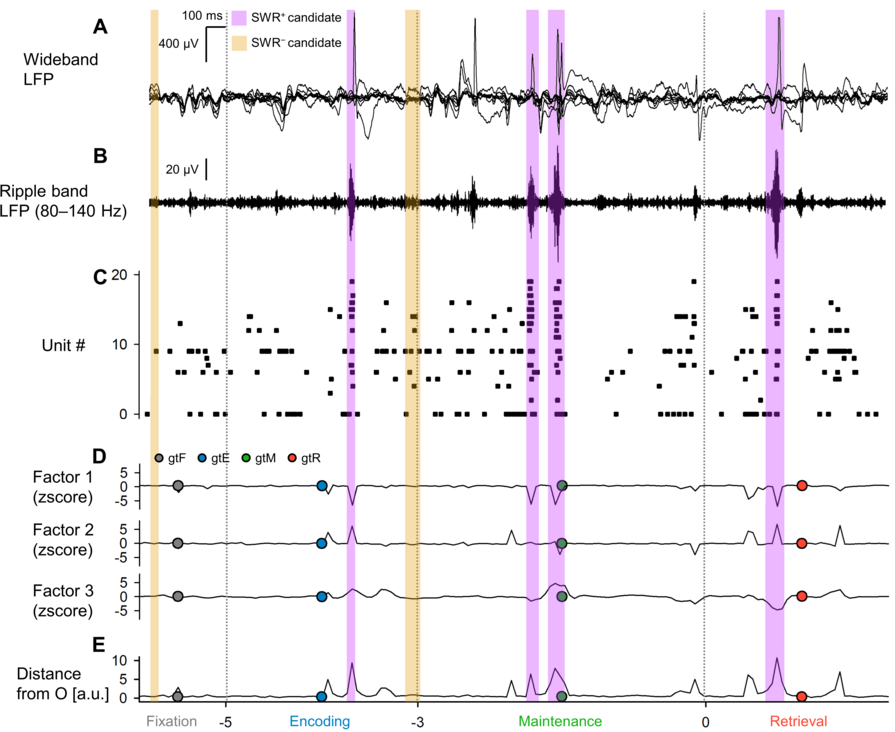
\includegraphics[width=1\textwidth]{./src/figures/.png/Figure_ID_01.png}
        	\caption{\textbf{Local Field Potential (LFP), Multiunit Activity, and Neural Trajectory of the Hippocampus during a Modified Sternberg Task} \cite{li_functional_2023, borders_hippocampal_2022, dimakopoulos_information_2022}}
\smallskip
\\
\textbf{\textit{A.}} This segment presents representative wideband LFP traces from iEEG signals, observed in the left hippocampal head throughout the completion of a modified Sternberg working memory task. The task involves fixation (1 s, \textit{gray}), encoding (2 s, \textit{blue}), maintenance (3 s, \textit{green}), and retrieval (2 s, \textit{red}) \cite{li_functional_2023, borders_hippocampal_2022, dimakopoulos_information_2022}. \textbf{\textit{B.}} The corresponding ripple band LFP traces are depicted here \cite{schomburg_spiking_2012, behrens_induction_2005, norimoto_hippocampal_2018}. \textbf{\textit{C.}} The raster plot of multiunit spikes, derived from the LFP traces utilizing a spike sorting algorithm, is illustrated here \cite{niediek_reliable_2016}. \textbf{\textit{D.}} This part represents the neural trajectory, established by the GPFA, computed from the spike counts per unit within 50-ms bins \cite{yu_gaussian-process_2009}. The dotted circles represent the geometric median coordinates for each phase. \textbf{\textit{E.}} The distance from the trajectory to the point $O$ is demonstrated here. It is notable that the \textit{purple} and \textit{yellow} rectangles denote the timings for SWR$^+$ candidates and SWR$^-$ candidates, respectively, functioning as controls for SWR$^+$ \cite{van_vugt_hippocampal_2010, scoville_loss_1957, kay_hippocampal_2016, nader_memory_2003, wilson_reactivation_1994, nadasdy_replay_1999, lee_memory_2002}.
}
% width=1\textwidth
        	\label{fig:01}
        \end{figure*}
        \clearpage
        \begin{figure*}[ht]
            \pdfbookmark[2]{ID 02}{figure_id_02}
        	\centering
            \includegraphics[width=]{./src/figures/.png/Figure_ID_02.png}
        	\caption{\textbf{
State-dependent Hippocampal Neural Trajectory
}
\smallskip
\\
\textbf{\textit{A.}} This figure presents the neural trajectory within the first three dimensions, derived using Gaussian Process Factor Analysis (GPFA). Each smaller dot signifies the coordinates of a 50-ms neural trajectory bin, while larger dots indicated in \textit{black} represent the geometric medians of successive phases in the Sternberg working memory task. The phases include fixation (\textit{gray}), encoding (\textit{blue}), maintenance (\textit{green}), and retrieval (\textit{red})\cite{yu_gaussian-process_2009}. \textbf{\textit{B.}} The graph shows the log-likelihood of GPFA models compared to the number of dimensions employed for embedding multi-unit spikes within medial temporal lobe (MTL) regions. Notably, the optimal dimensionality was found to be three, based on the elbow method\cite{virtanen_scipy_2020}. \textbf{\textit{C.}} This section delineates the distance between the neural trajectory and the origin ($O$) for the hippocampus (Hipp.), entorhinal cortex (EC), and amygdala (Amy.), and plots it over time since the onset of the probe \cite{boran_dataset_2020}. \textbf{\textit{D.}} The subsequent graph underscores the trajectory's distance from $O$ across MTL regions, with the hippocampus registering the most extensive distance, followed by the EC and Amygdala\cite{fernandez-ruiz_long-duration_2019}. \textbf{\textit{E.}} The final depiction signifies the inter-phase trajectory distances within the MTL regions\cite{liu_consensus_2022}.
Abbreviations:
}
        	\label{fig:02}
        \end{figure*}
        \clearpage
        \begin{figure*}[ht]
            \pdfbookmark[2]{ID 03}{figure_id_03}
        	\centering
            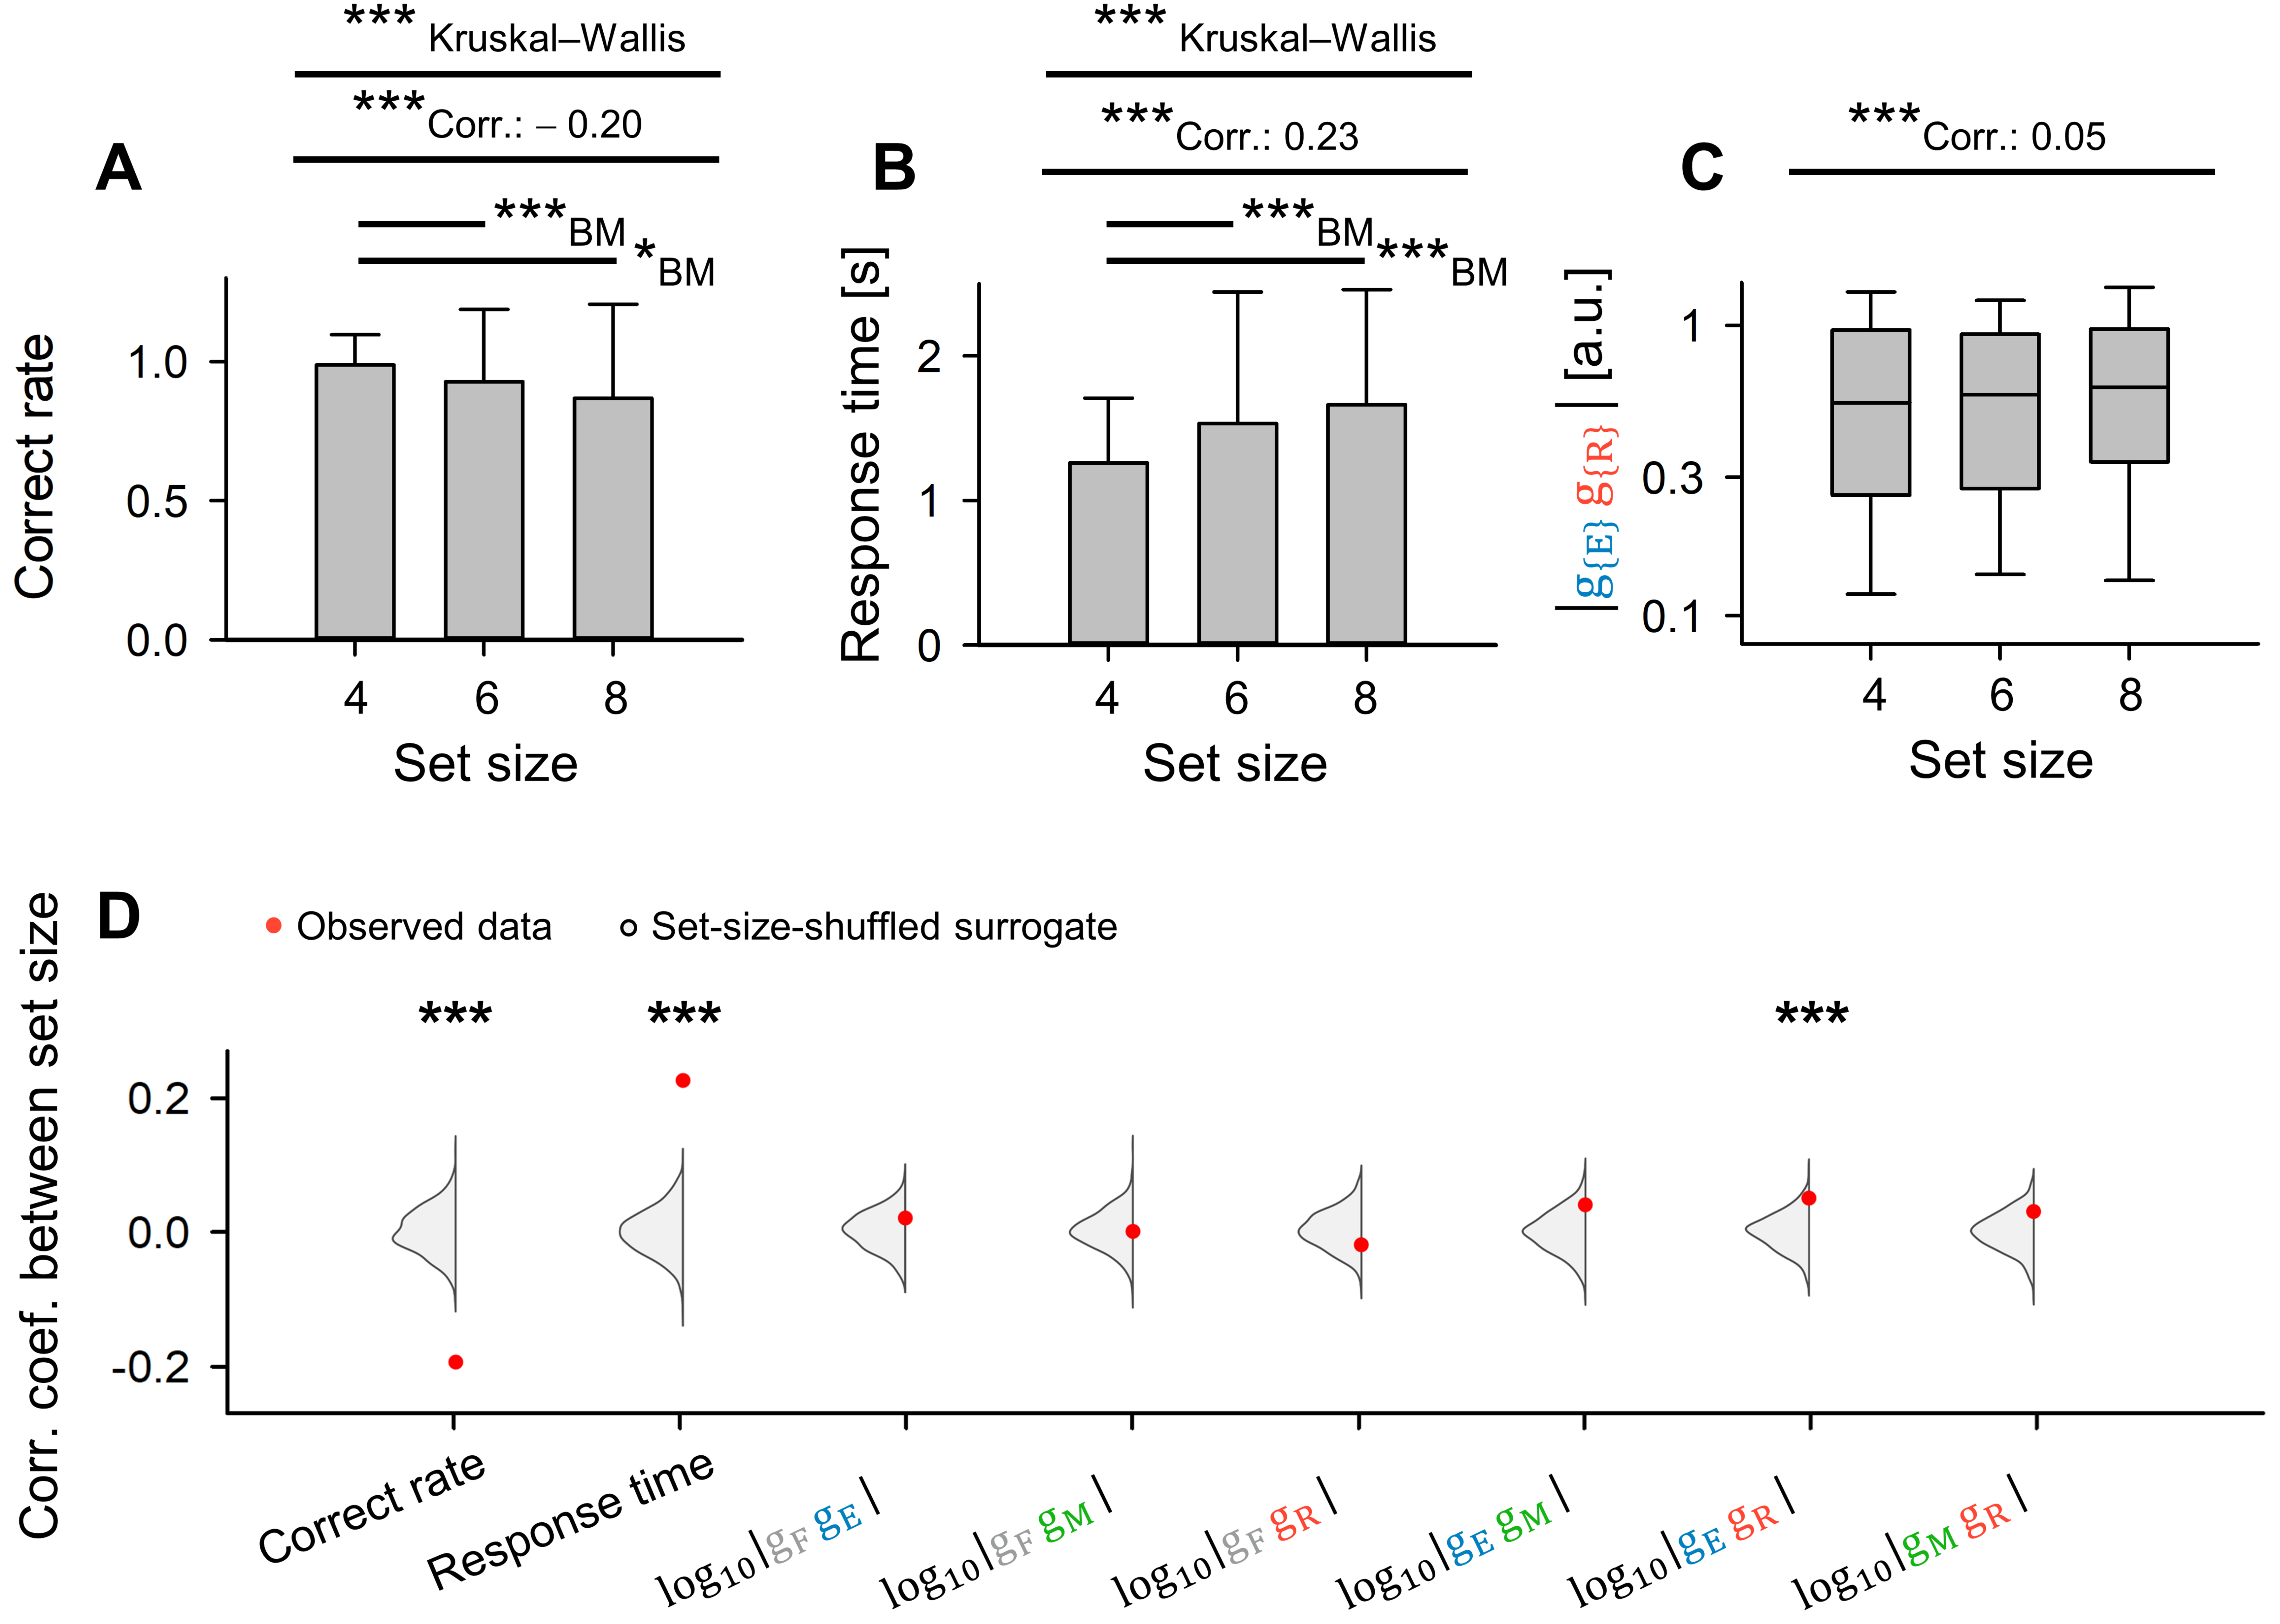
\includegraphics[width=1\textwidth]{./src/figures/.png/Figure_ID_03.png}
        	\caption{\textbf{
Dependence of Trajectory Distance on Memory Load Between Encoding and Retrieval States in the Hippocampus
}
\smallskip
\\
\textbf{\textit{A.}} A significant correlation has been documented between the set size (the number of letters to encode) and the correctness rate in the WM task (coefficient = $-0.20$, ***\textit{p} $<$ 0.001) \cite{van_vugt_hippocampal_2010, li_functional_2023, borders_hippocampus_2022}. \textbf{\textit{B.}} A notable correlation exists between set size and response time (coefficient = $0.23$, ***\textit{p} $<$ 0.001) \cite{dimakopoulos_information_2022}.  \textbf{\textit{C.}} There is a correlation between set size and the distances between encoding and retrieval phases ($\Vert \mathrm{g_{E}g_{R}} \Vert$), but it's less significant (correlation coefficient = 0.05) \cite{li_functional_2023}. \textbf{\textit{D.}} \textit{Red} dots express the observed correlations between set size and the stated parameters: correct rate, response time, $\log_{10}{\Vert \mathrm{g_{F}g_{E}} \Vert}$, $\log_{10}{\Vert \mathrm{g_{F}g_{M}} \Vert}$, $\log_{10}{\Vert \mathrm{g_{F}g_{R}} \Vert}$, $\log_{10}{\Vert \mathrm{g_{E}g_{M}} \Vert}$, $\log_{10}{\Vert \mathrm{g_{E}g_{R}} \Vert}$, and $\log_{10}{\Vert \mathrm{g_{M}g_{R}} \Vert}$. The \textit{gray} kernel density plot illustrates the corresponding randomized set-size measurements (\textit{n} = 1,000) (***\textit{p}s $<$ 0.001) \cite{norimoto_hippocampal_2018, hajos_input-output_2013}.
}
% width=1\textwidth
        	\label{fig:03}
        \end{figure*}
        \clearpage
        \begin{figure*}[ht]
            \pdfbookmark[2]{ID 04}{figure_id_04}
        	\centering
            \includegraphics[width=1\textwidth]{./src/figures/.png/Figure_ID_04.png}
        	\caption{\textbf{Detection of SWRs in Presumed CA1 Regions}
\smallskip
\\
\textbf{\textit{A.}} A two-dimensional Uniform Manifold Approximation and Projection (UMAP) projection of multi-unit spikes during potential SWRs (\textit{purple}) and non-SWRs (\textit{yellow}) periods is given\cite{mcinnes_umap_2018}. \textbf{\textit{B.}} The cumulative density plot of silhouette scores, measuring the quality of UMAP clustering across diverse hippocampal regions, is shown (refer to Table~\ref{tab:02}). Regions that attained a silhouette score above 0.60 (corresponding to the $75^{th}$ percentile), are identified as probable CA1 areas. Within these potential CA1 regions, the SWR and non-SWR periods were respectively categorized as SWRs and non-SWRs (\textit{n} = 1,170)\cite{rousseeuw_silhouettes_1987}. \textbf{\textit{C.}} The distributions of durations for both SWRs (\textit{purple}) and non-SWRs (\textit{yellow}) are depicted, based on their respective definitions (93.0 [65.4] ms, median [IQR])\cite{girardeau_selective_2009}\cite{norman_hippocampal_2021}. \textbf{\textit{D.}} An illustration of the frequency of SWRs (\textit{purple}) and non-SWRs (\textit{yellow}) over time from the start of stimulation, represented by mean value \textpm 95\% confidence interval is given. It should be noted that due to close intervals, visual differentiation can be difficult. Additionally, there was a discernible increase in SWR frequency during the initial 400 ms of the retrieval phase (0.421 [Hz], *\textit{p} < 0.05, bootstrap test)\cite{buzsaki_hippocampal_2015}\cite{ego-stengel_disruption_2010}\cite{fernandez-ruiz_long-duration_2019}. \textbf{\textit{E.}} Distributions of ripple band peak amplitudes for non-SWRs (\textit{yellow}; 2.37 [0.33] times the standard deviation (SD) of the baseline, median [IQR]) and SWRs (\textit{purple}; 3.05 [0.85] times the SD of the baseline, median [IQR]) are exhibited. Considerable differences were observed (***\textit{p} < 0.001, by the Brunner--Munzel test)\cite{norman_hippocampal_2019}\cite{diba_forward_2007}\cite{liu_consensus_2022}.
}
% width=1\textwidth
        	\label{fig:04}
        \end{figure*}
        \clearpage
        \begin{figure*}[ht]
            \pdfbookmark[2]{ID 05}{figure_id_05}
        	\centering
            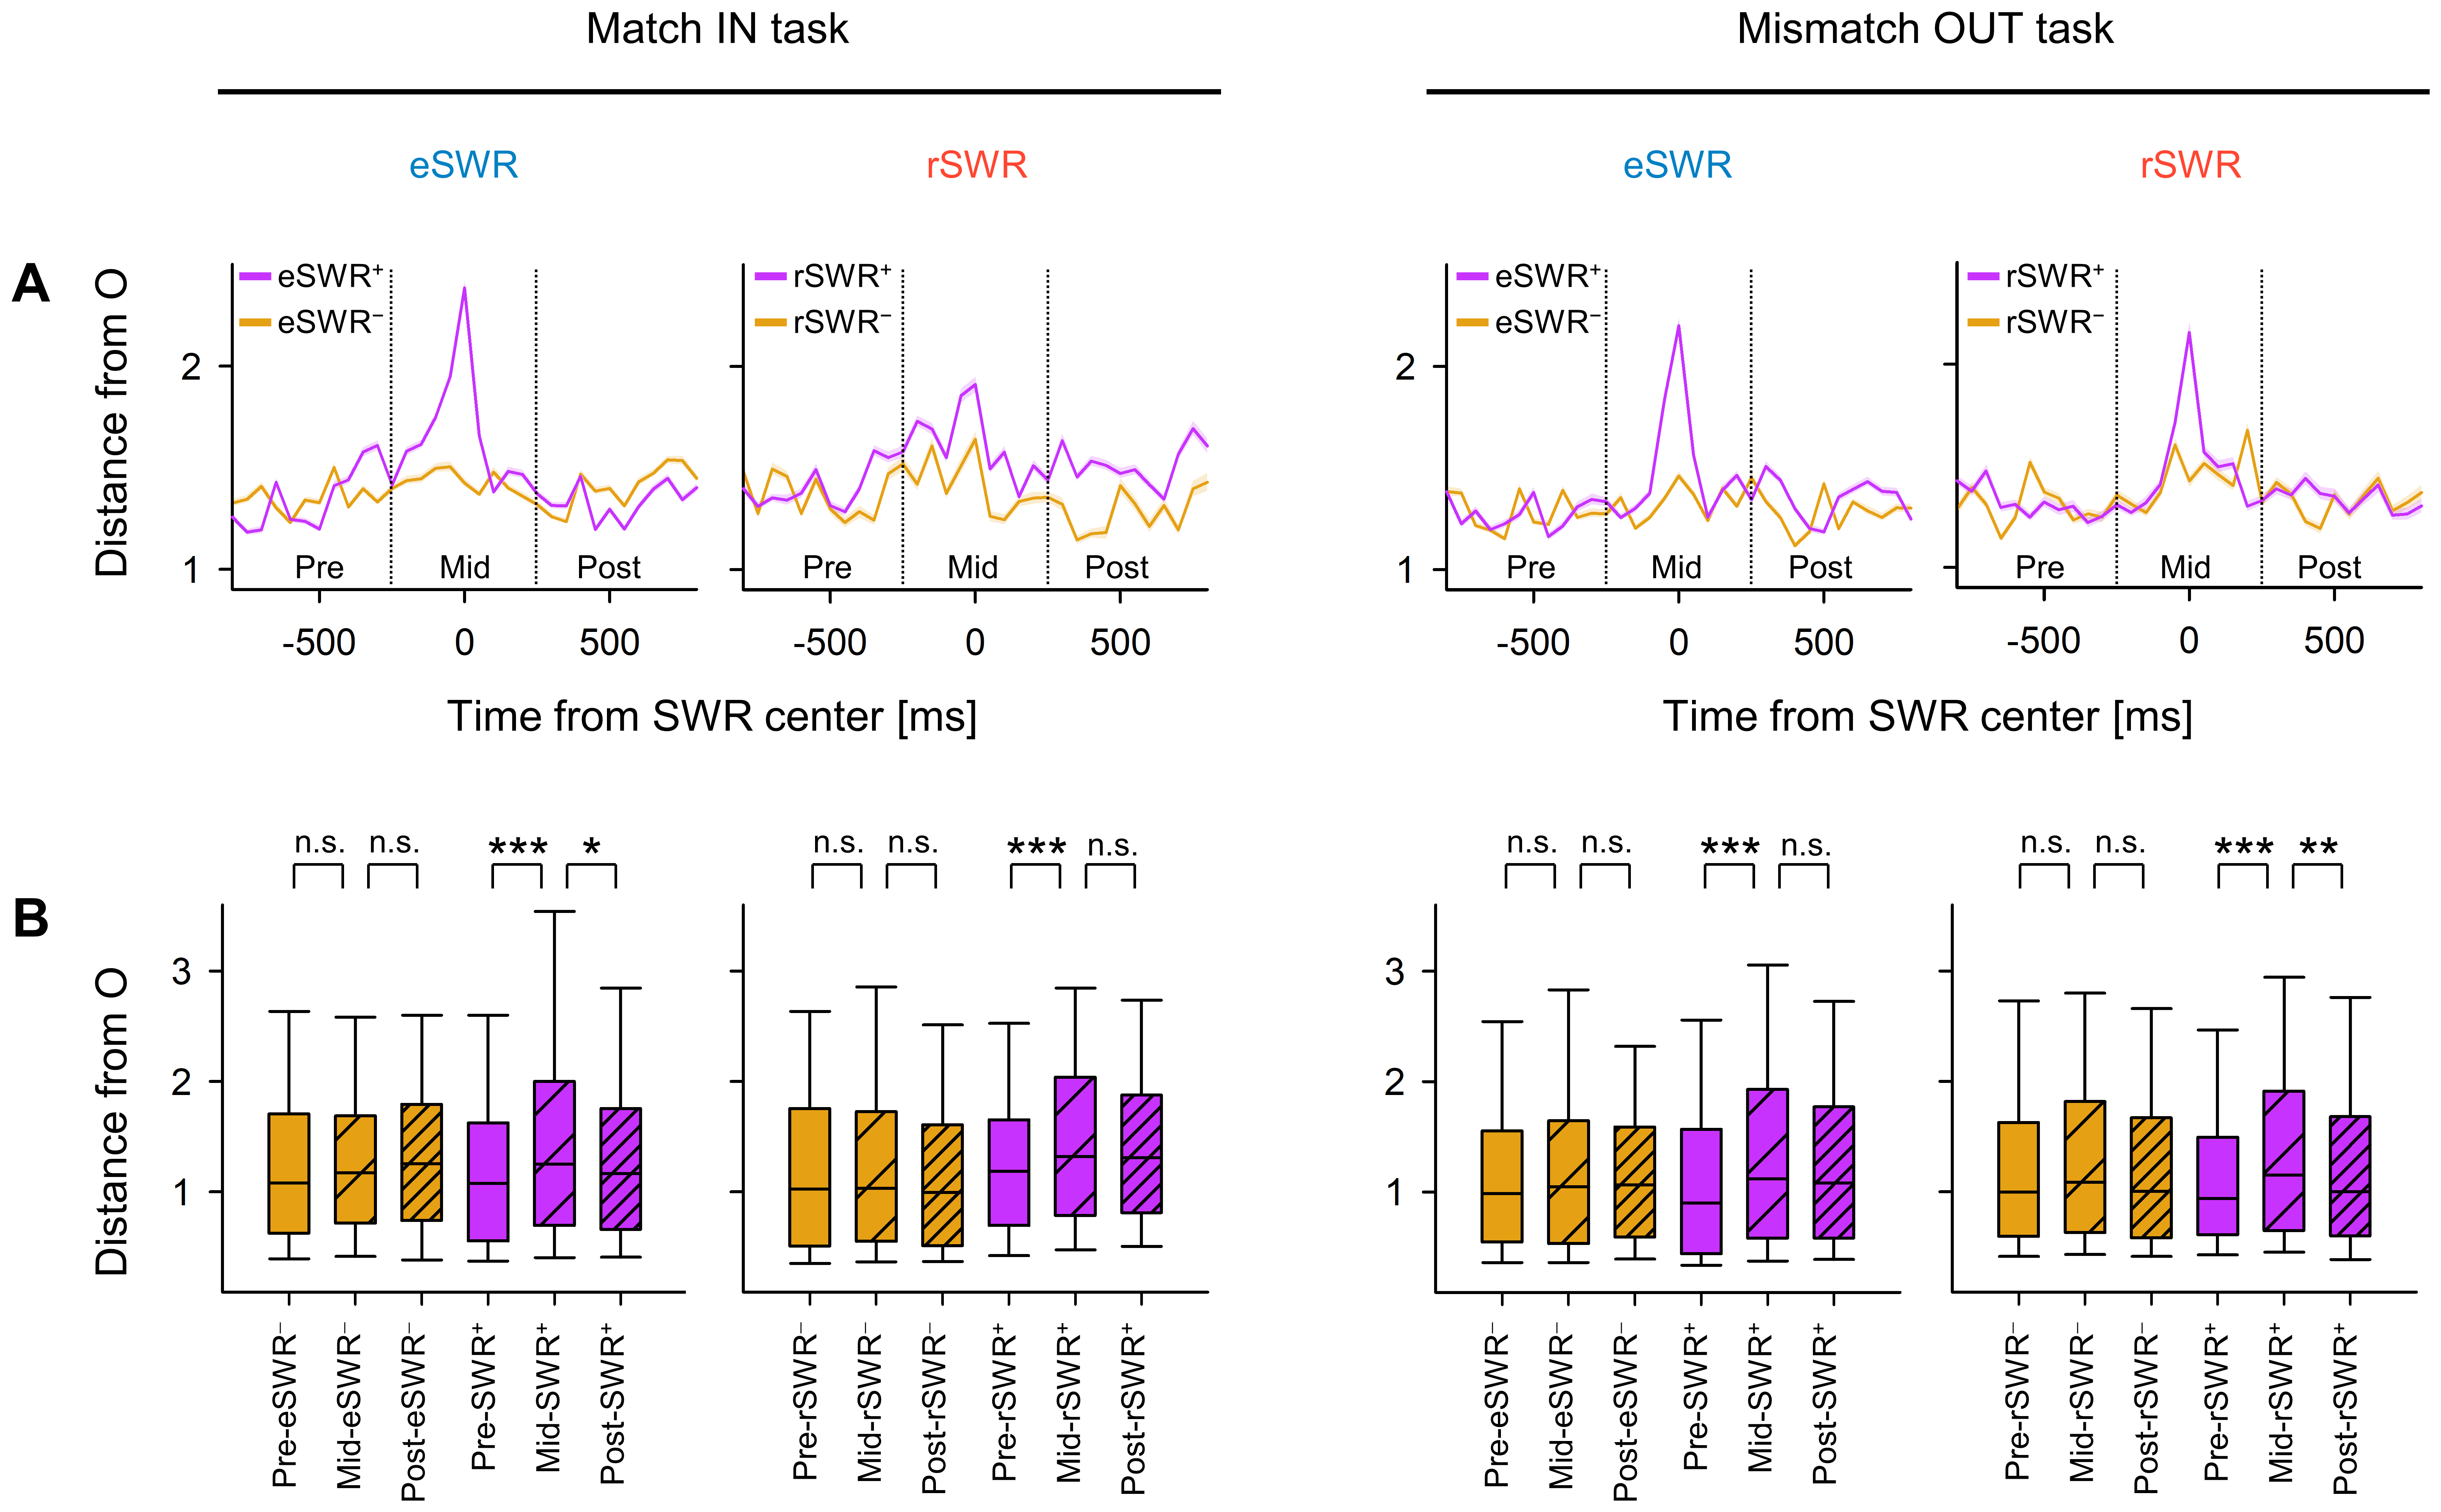
\includegraphics[width=1\textwidth]{./src/figures/.png/Figure_ID_05.png}
        	\caption{\textbf{Transient Changes in Neural Trajectory During SWR}}
\smallskip
\\
\textbf{\textit{A.}} Depicts the average distance from the origin ($O$) of the peri-sharp-wave-ripple (SWR) trajectory, alongside a 95\% confidence interval, which may not be evident due to its limited range \cite{girardeau_selective_2009,norman_hippocampal_2019,buzsaki_hippocampal_2015}. \textbf{\textit{B.}} Demonstrates the distance from the origin ($O$) throughout pre-, mid-, and post-SWR intervals (*\textit{p} $<$ 0.05, **\textit{p} $<$ 0.01, ***\textit{p} $<$ 0.001; according to the Brunner--Munzel test \cite{boran_persistent_2019}). The defined terms are: SWR, sharp-wave ripple events; eSWR, SWR occurring during the encoding phase; rSWR, SWR taking place during the retrieval phase; SWR$^+$, an SWR event; SWR$^-$, the control events aligned with SWR$^+$; pre-, mid-, or post-SWR, the time segments from $-800$ to $-250$ ms, from $-250$ to $+250$ ms, and from $+250$ to $+800$ ms, respectively, each relative to the SWR center.
}
% width=1\textwidth
        	\label{fig:05}
        \end{figure*}
        \clearpage
        \begin{figure*}[ht]
            \pdfbookmark[2]{ID 06}{figure_id_06}
        	\centering
            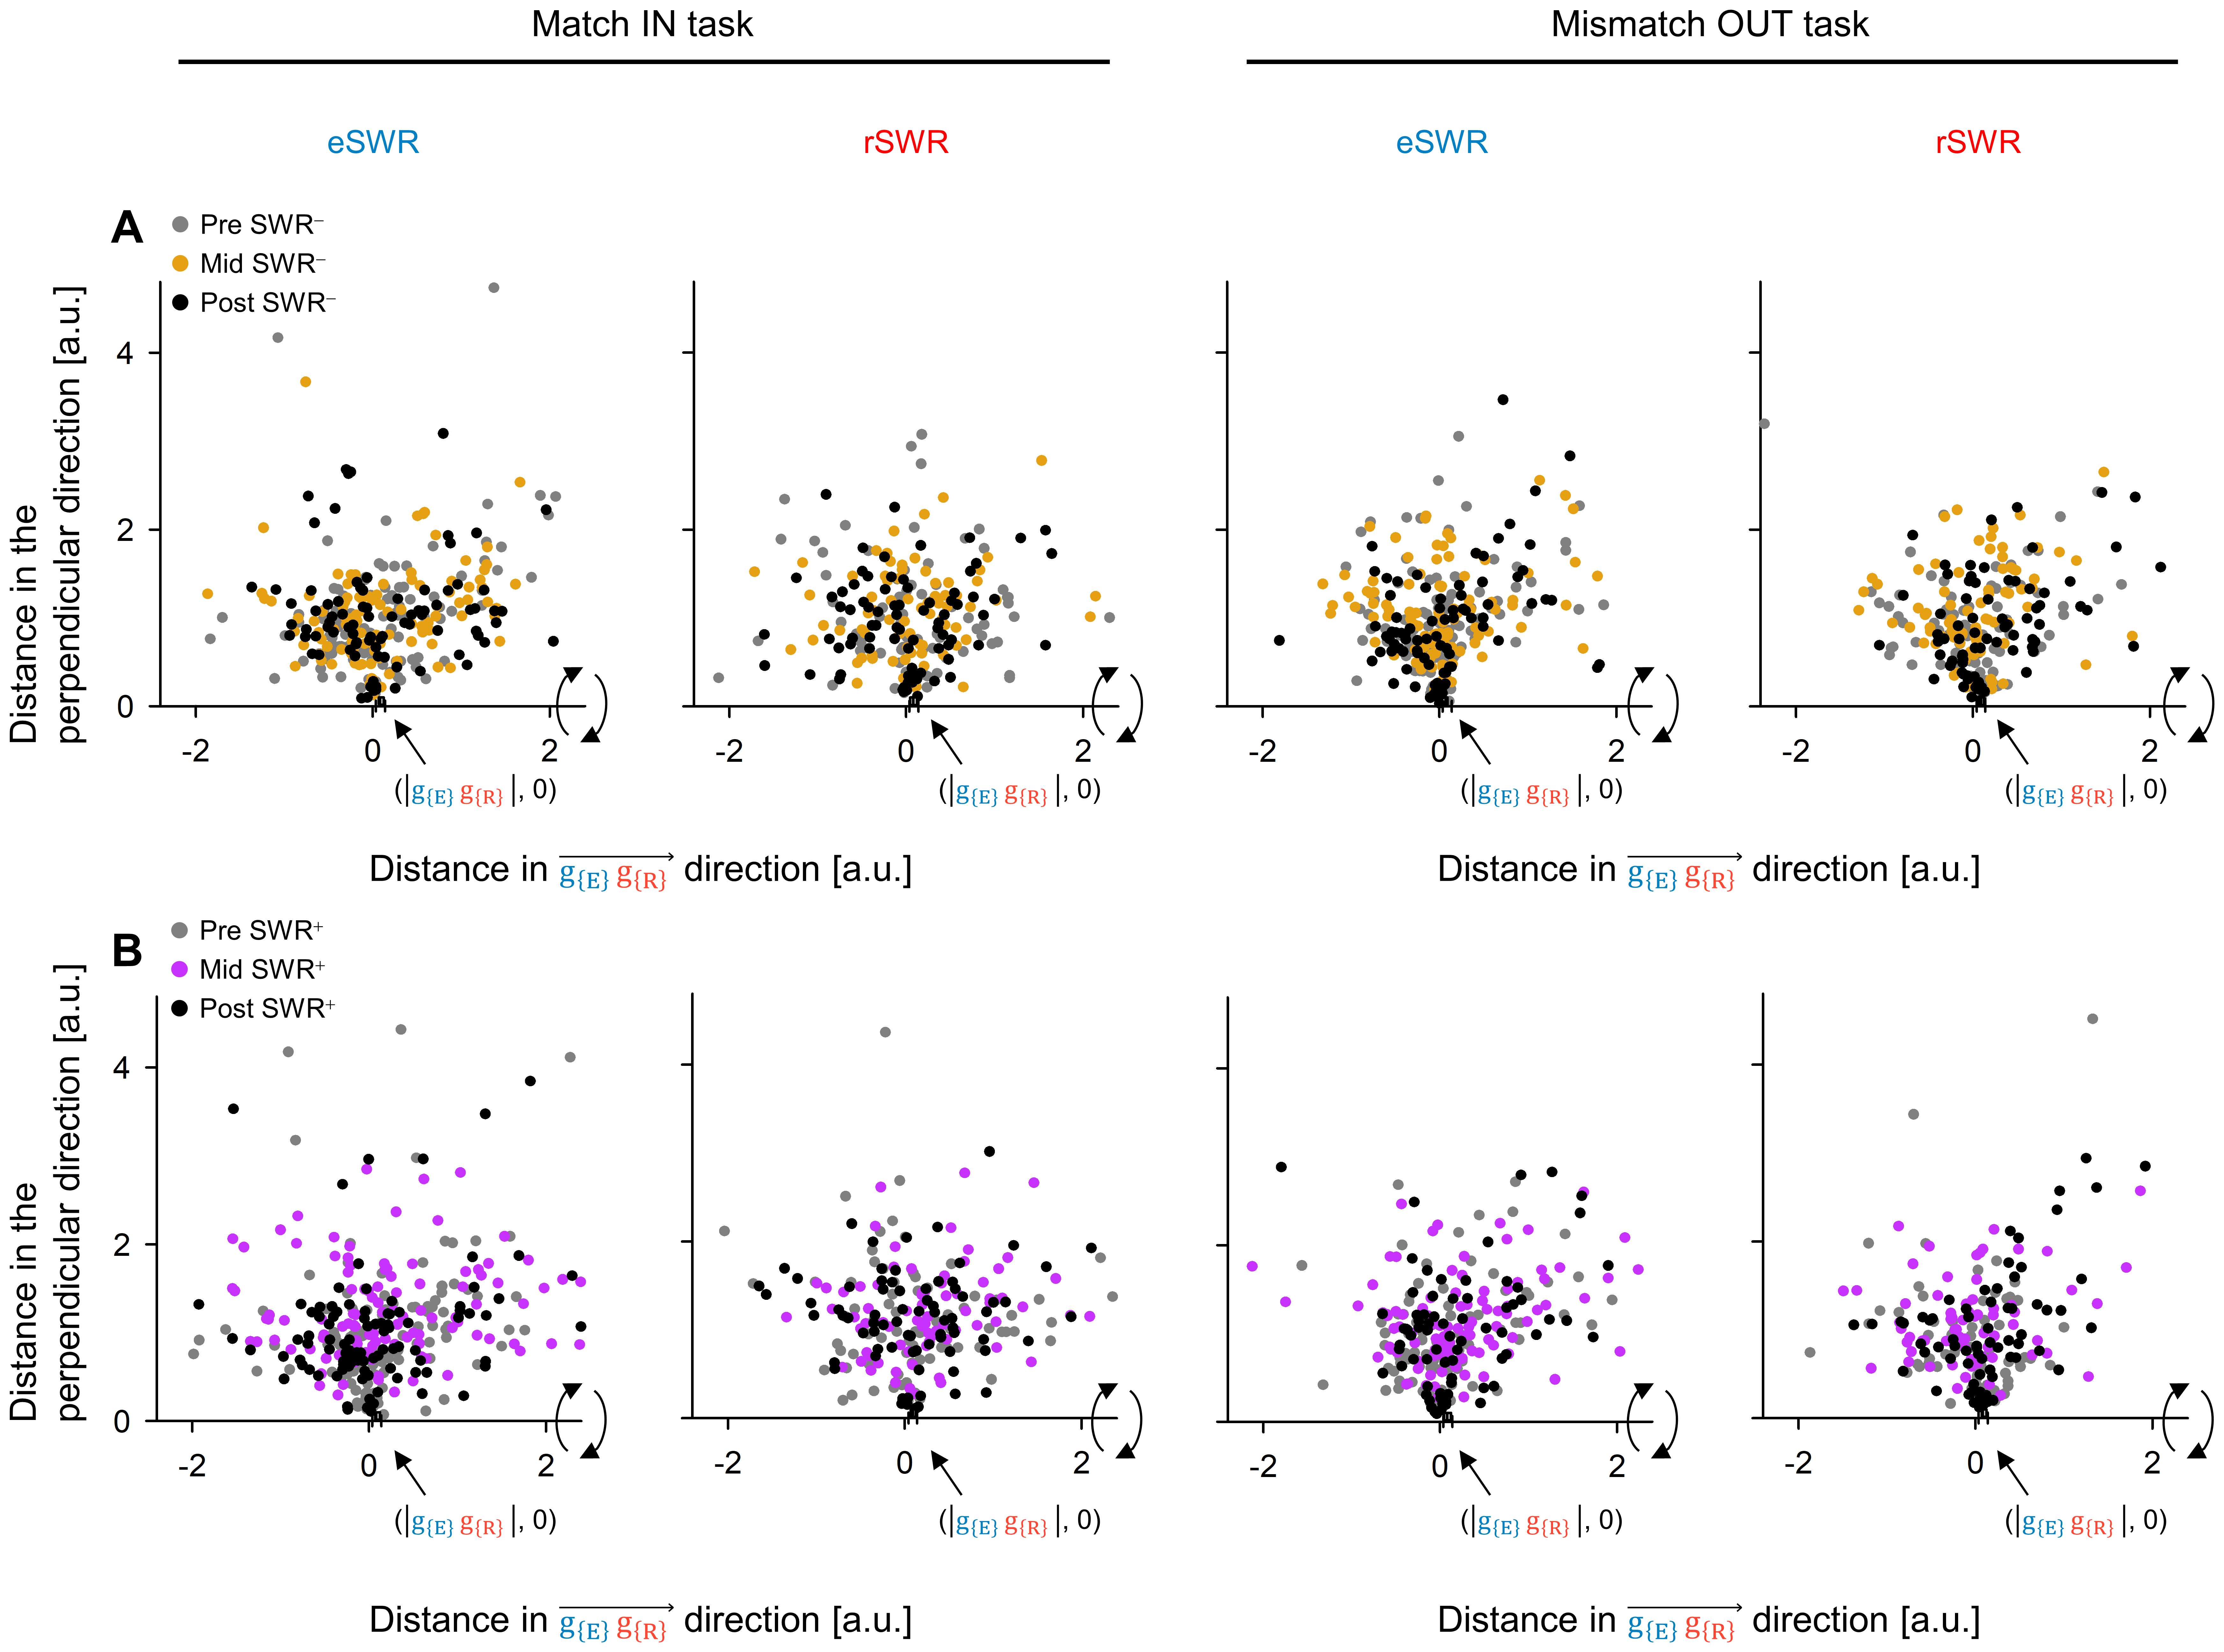
\includegraphics[width=1\textwidth]{./src/figures/.png/Figure_ID_06.png}
        	\caption{\textbf{Visualizing Neural Trajectories During Sharp-Wave Ripple Events in a Two-Dimensional Space}

\smallskip

\\
This figure demonstrates the association of neural trajectories with hippocampal activity during Sharp-Wave Ripple (SWR) events in a two-dimensional context. \textbf{\textit{A.}} It depicts example trajectories of the pre- (\textit{gray}), mid- (\textit{yellow}), and post-SWR$^-$ (\textit{black}) phases of an SWR event~\cite{buzsaki_hippocampal_2015}. \textbf{\textit{B.}} The trajectories that correspond with SWR$^+$ conditions are presented, contrasting with the SWR$^-$ backdrop~\cite{fernandez-ruiz_long-duration_2019}. Variations in the magnitude of $\lVert \mathrm{g_{E}g_{R}} \rVert$ are evident across sessions~\cite{liu_consensus_2022}. The projection protocol is outlined as follows: initially, $\mathrm{g_{E}}$ was located at the origin $O$ (0,0) and $\mathrm{g_{R}}$ at ($\lVert \mathrm{g_{E}g_{R}} \rVert$, 0), realized through linear transformation~\cite{kim_corticalhippocampal_2022}. Subsequently, rotation of the point cloud around the $\mathrm{g_{E}g_{R}}$ axis (the x-axis) was conducted to accommodate a two-dimensional space~\cite{yu_gaussian-process_2009}. As a result, the distances from $O$ and the angles relative to the $\mathrm{g_{E}g_{R}}$ axis remained consistent with their original three-dimensional configuration~\cite{mcinnes_umap_2018}. Key terms used in this context: SWR pertains to Sharp-Wave Ripple events; eSWR means SWR during the encoding phase; rSWR signifies SWR during the retrieval phase; SWR$^+$ defines an SWR event; SWR$^-$ represents the control event for SWR$^+$; pre-SWR, mid-SWR, and post-SWR indicate time intervals from $-800$ to $-250$ ms, from $-250$ to $+250$ ms, and from $+250$ to $+800$ ms from the center of an SWR event, respectively~\cite{zhang_hippocampal_2022}.
}
% width=1\textwidth
        	\label{fig:06}
        \end{figure*}
        \clearpage
        \begin{figure*}[ht]
            \pdfbookmark[2]{ID 07}{figure_id_07}
        	\centering
            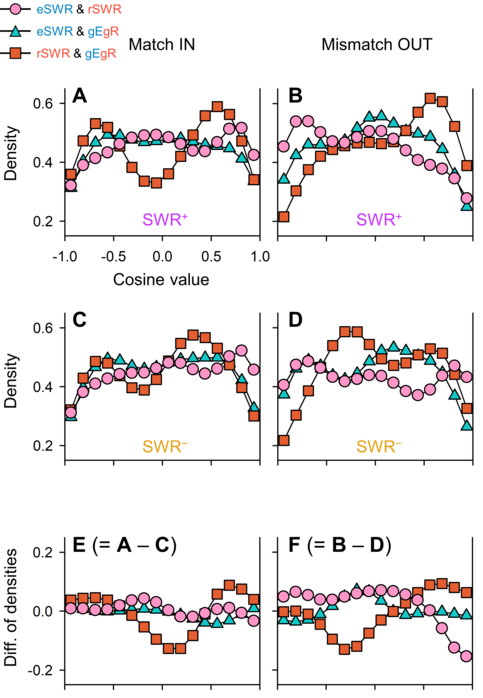
\includegraphics[width=0.5\textwidth]{./src/figures/.png/Figure_ID_07.png}
        	\caption{\textbf{
Directionality of Neural Trajectories in SWR Based on Encoding and Retrieval States
}
\smallskip
\\
\textbf{\textit{A--B}} Depicted are the Kernel Density Estimation (KDE) distributions of $\protect\overrightarrow{{\mathrm{eSWR^+}}} \cdot \protect\overrightarrow{{\mathrm{rSWR^+}}}$ (\textit{pink circles}), $\protect\overrightarrow{{\mathrm{eSWR^+}}} \cdot \protect\overrightarrow{{\mathrm{g_{E}g_{R}}}}$ (\textit{blue triangles}), and $\protect\overrightarrow{{\mathrm{rSWR^+}}} \cdot \protect\overrightarrow{{\mathrm{g_{E}g_{R}}}}$ (\textit{red rectangles}) in Match IN (\textit{A}) and Mismatch OUT tasks (\textit{B})~\cite{li_functional_2023}. \textbf{\textit{C--D}} Similar distributions for these tasks where $\mathrm{SWR^-}$ replaces $\mathrm{SWR^+}$ have been presented~\cite{dimakopoulos_information_2022}. \textbf{\textit{E--F}} Distinctions between the distributions of $\mathrm{SWR^+}$ and $\mathrm{SWR^-}$ highlight the SWR components (\textit{E} = \textit{C} $-$ \textit{A}; \textit{F} = \textit{D} $-$ \textit{B}), where the biphasic distributions of $\protect\overrightarrow{{\mathrm{rSWR^-}}} \cdot \protect\overrightarrow{{\mathrm{g_{E}g_{R}}}}$ indicate neural oscillations between encoding and retrieval states during the Sternberg task~\cite{borders_hippocampus_2022}. Contrarily, the Mismatch OUT task showed an inverse relationship between $\protect\overrightarrow{{\mathrm{eSWR^+}}}$ and $\protect\overrightarrow{{\mathrm{rSWR^+}}}$ (\textit{pink circles}), a finding not observed in the Match IN task (\textbf{\textit{E--F}})~\cite{naber_reciprocal_2001,van_strien_anatomy_2009}. Lastly, transitions from retrieval to encoding for the SWR components were apparent in both Match IN and Mismatch OUT tasks (\textit{red rectangles} in \textit{E--F})~\cite{niediek_reliable_2016,schomburg_spiking_2012}.
}
% width=0.5\textwidth
        	\label{fig:07}
        \end{figure*}


%%%%%%%%%%%%%%%%%%%%%%%%%%%%%%%%%%%%%%%%%%%%%%%%%%%%%%%%%%%%%%%%%%%%%%%%%%%%%%%%
%% END
%%%%%%%%%%%%%%%%%%%%%%%%%%%%%%%%%%%%%%%%%%%%%%%%%%%%%%%%%%%%%%%%%%%%%%%%%%%%%%%%

\end{document}
